\documentclass[a4paper,12pt]{article}
\usepackage[top = 2.5cm, bottom = 2.5cm, left = 2.5cm, right = 2.5cm]{geometry}
\usepackage[T1]{fontenc}
\usepackage[utf8]{inputenc}
\usepackage{multirow} 
\usepackage{booktabs} 
\usepackage{graphicx}
\usepackage[spanish]{babel}
\usepackage{setspace}
\setlength{\parindent}{0in}
\usepackage{float}
\usepackage{fancyhdr}
\usepackage{amsmath}
\usepackage{amssymb}
\usepackage{amsthm}
\usepackage[numbers]{natbib}
\newcommand\Mycite[1]{%
	\citeauthor{#1}~[\citeyear{#1}]}
\usepackage{graphicx}
\usepackage{subcaption}
\usepackage{booktabs}
\usepackage{etoolbox}
\usepackage{minibox}
\usepackage{hyperref}
\usepackage{xcolor}
\usepackage[skins]{tcolorbox}
%---------------------------

\newtcolorbox{cajita}[1][]{
	 #1
}

\newenvironment{sol}
{\renewcommand\qedsymbol{$\square$}\begin{proof}[\textbf{Solución.}]}
	{\end{proof}}

\newenvironment{dem}
{\renewcommand\qedsymbol{$\blacksquare$}\begin{proof}[\textbf{Demostración.}]}
	{\end{proof}}

\newtheorem{problema}{Problema}
\newtheorem{variable}{Variable}
\newtheorem{definicion}{Definición}
\newtheorem{ejemplo}{Ejemplo}
\newtheorem{teorema}{Teorema}
\newtheorem{corolario}{Corolario}[teorema]
\newtheorem{lema}[teorema]{Lema}
\newtheorem{prop}{Proposición}
\newtheorem*{nota}{\textbf{NOTA}}
\renewcommand\qedsymbol{$\blacksquare$}
\usepackage{svg}
\usepackage{tikz}
\usepackage[framemethod=default]{mdframed}
\global\mdfdefinestyle{exampledefault}{%
linecolor=lightgray,linewidth=1pt,%
leftmargin=1cm,rightmargin=1cm,
}




\newenvironment{noter}[1]{%
\mdfsetup{%
frametitle={\tikz\node[fill=white,rectangle,inner sep=0pt,outer sep=0pt]{#1};},
frametitleaboveskip=-0.5\ht\strutbox,
frametitlealignment=\raggedright
}%
\begin{mdframed}[style=exampledefault]
}{\end{mdframed}}
\newcommand{\linea}{\noindent\rule{\textwidth}{3pt}}
\newcommand{\linita}{\noindent\rule{\textwidth}{1pt}}

\AtBeginEnvironment{align}{\setcounter{equation}{0}}
\pagestyle{fancy}

\fancyhf{}









%----------------------------------------------------------
\lhead{\footnotesize Data Science I}
\rhead{\footnotesize  Alonso, Cuellar, Rompich}
\cfoot{\footnotesize \thepage}


%--------------------------

\begin{document}
 \thispagestyle{empty} 
    \begin{tabular}{p{15.5cm}}
    \begin{tabbing}
    \textbf{Universidad del Valle de Guatemala} \\\\
   \textbf{Estudiantes:} Augusto Alonso, David Cuellar, Rudik Rompich\\
   
   
   \textbf{Correos:}  \href{mailto:alo181085@uvg.edu.gt}{alo181085@uvg.edu.gt}, \href{mailto:cue18382@uvg.edu.gt}{cue18382@uvg.edu.gt},\href{mailto:rom19857@uvg.edu.gt}{rom19857@uvg.edu.gt}\\
   \textbf{Carnés:} 181085, 18382,19857
    \end{tabbing}
    \begin{center}
        CC3066 - Data Science I - Catedrático: Luis Furlan\\
        \today
    \end{center}\\
    \hline
    \\
    \end{tabular} 
    \vspace*{0.3cm} 
    \begin{center} 
    {\Large \bf  Code Book
} 
        \vspace{2mm}
    \end{center}
    \vspace{0.4cm}
%--------------------------


\section{Descripción general}

El resumen de las estadísticas de la base de datos se puede observar en \ref{fig: 1}, la división de tipo de variables se eligió arbitrariamente; colocando a todas las variables como categóricas (exceptuando al código). La base de datos contiene 18 variables y tiene 65021 filas de todos los centros educativos. 
	\begin{figure}[H]
	\centering
	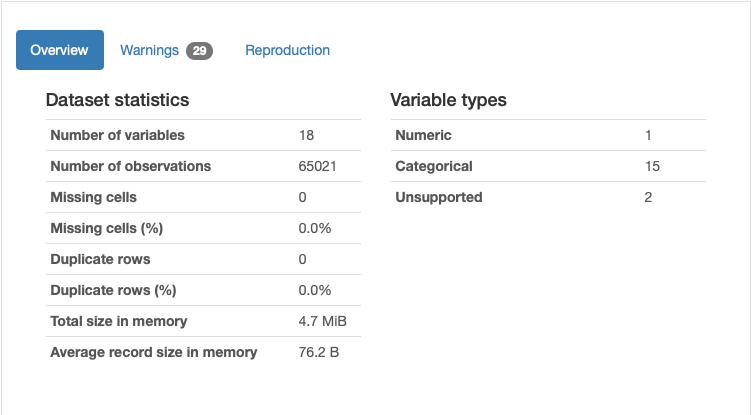
\includegraphics[scale=0.5]{Images/0}
	\caption{Resumen}
	\label{fig: 1}
\end{figure}

\newpage

\section{Descripción de variables}

\begin{variable}(codigo) 
	La variable código sirve para identificar cada establecimiento educativo por un índice único. 
	\bigbreak 
	\textbf{Valores posibles.}
	\begin{itemize}
		\item 65021 índices distintos, representando a todos los centros educativos. 
	\end{itemize}
	\begin{figure}[H]
		\centering
		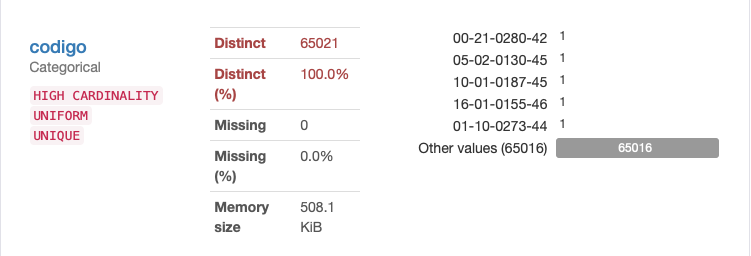
\includegraphics[scale=0.5]{Images/1}
	\end{figure}
\end{variable}

%-

\begin{variable}(distrito) 
	Hace referencia al distrito donde se encuentra el centro educativo. Su utilidad se encuentra en que representa al distrito de supervisión al que se encuentra regido. 
	\bigbreak 
	\textbf{Valores posibles.}
	\begin{itemize}
		\item 905 valores posibles. 
		\item 3928 valores nulos.
	\end{itemize}
	\begin{figure}[H]
		\centering
		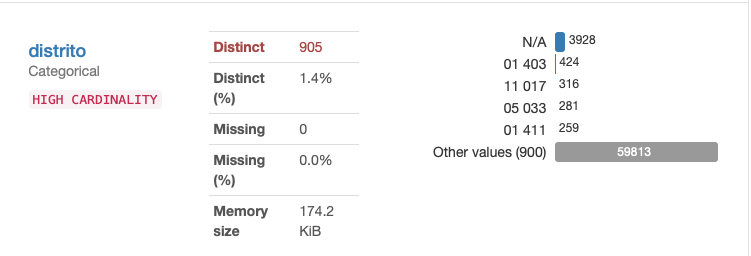
\includegraphics[scale=0.5]{Images/2}
	\end{figure}
\end{variable}

%-

\begin{variable}(departamento) 
Es la variable que representa al departamento en donde se encuentra el centro educativo.
\bigbreak 
\textbf{Valores posibles.}
\begin{itemize}
	\item Los 22 departamentos del país. 
\end{itemize}
\begin{figure}[H]
	\centering
	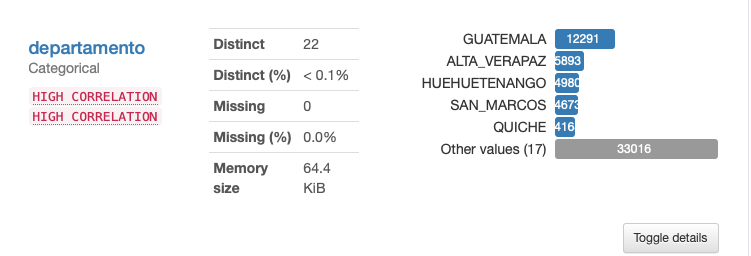
\includegraphics[scale=0.5]{Images/3}
\end{figure}
\end{variable}

%-

\begin{variable}(municipio) 
Es la variable que representa al municipio en donde se encuentra el centro educativo.
\bigbreak 
\textbf{Valores posibles.}
\begin{itemize}
	\item Los 357 departamentos del país. 
\end{itemize}
\begin{figure}[H]
	\centering
	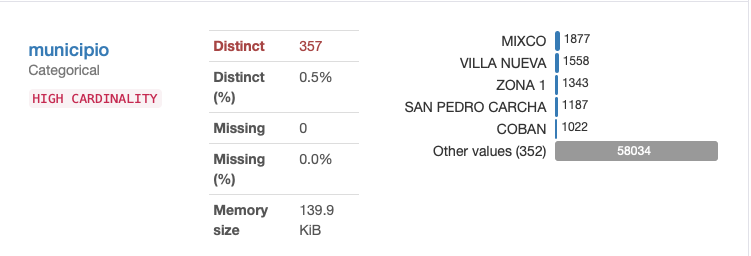
\includegraphics[scale=0.5]{Images/4}
\end{figure}
\end{variable}

%-

\begin{variable}(establecimiento) 
	Es una variable que hace referencia al nombre de los centros educativos y el tipo de centro educativo (mixto, urbana, rural, por cooperativa, telesecundaria). Los datos muestran que existen muchos centros educativos con el mismo nombre. 
\bigbreak 
\textbf{Valores posibles.}
\begin{itemize}
	\item 17452 centros educativos distintos. 
\end{itemize}
\begin{figure}[H]
	\centering
	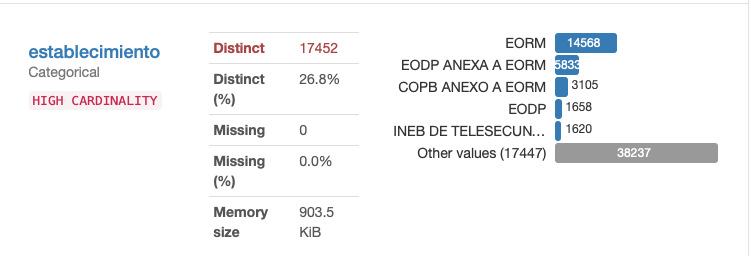
\includegraphics[scale=0.5]{Images/5}
\end{figure}
\end{variable}

%-

\begin{variable}(supervisor) 
Hace referencia al nombre de la persona que está encargada de la supervisión de los centros educativos. 
\bigbreak 
\textbf{Valores posibles.}
\begin{itemize}
	\item Existen 828 datos distintos.  
\end{itemize}
\begin{figure}[H]
	\centering
	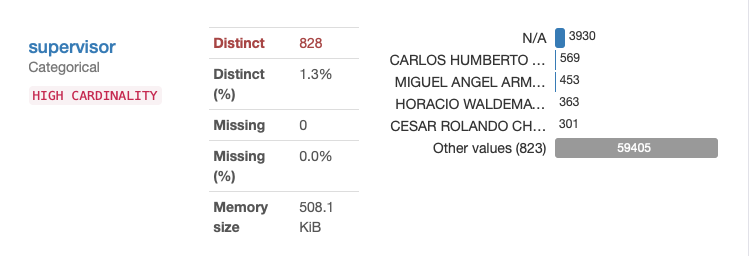
\includegraphics[scale=0.5]{Images/6}
\end{figure}
\end{variable}

%-

\begin{variable}(director) 
Es una variable que indica el nombre del director del centro educativo. 
\bigbreak 
\textbf{Valores posibles.}
\begin{itemize}
	\item La mayoría son valores nulos (pendiente de limpieza ). 
\end{itemize}
\begin{figure}[H]
	\centering
	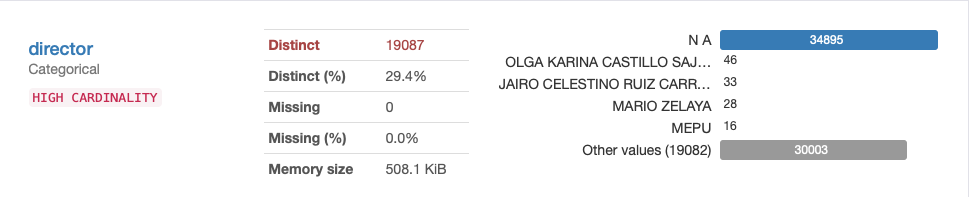
\includegraphics[scale=0.5]{Images/7}
\end{figure}
\end{variable}

%-

\begin{variable}(nivel) 
Es una variable que representa todos los niveles educativos que ofrecen los centros educativos.
\bigbreak 
\textbf{Valores posibles.}
\begin{itemize}
	\item 7 valores distintos (desde primaria hasta diversificado). 
\end{itemize}
\begin{figure}[H]
	\centering
	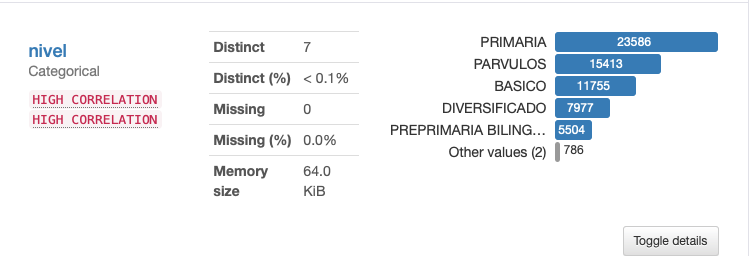
\includegraphics[scale=0.5]{Images/8}
\end{figure}
\end{variable}

%-

\begin{variable}(sector) 
Es una variable que complementa a la variable de establecimiento ya que separa en una columna específica el tipo de centro de educativo que representa.
\bigbreak 
\textbf{Valores posibles.}
\item 5 valores distintos. 
\begin{itemize}
	\item 
\end{itemize}
\begin{figure}[H]
	\centering
	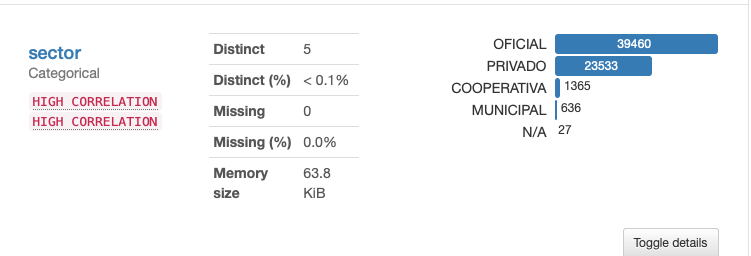
\includegraphics[scale=0.5]{Images/9}
\end{figure}
\end{variable}

%-

\begin{variable}(area) 
Es una variable que complementa a la variable de establecimiento ya que separa en una columna específica la locación de centro de educativo.
\bigbreak 
\textbf{Valores posibles.}
\begin{itemize}
	\item 4 valores distintos. 
\end{itemize}
\begin{figure}[H]
	\centering
	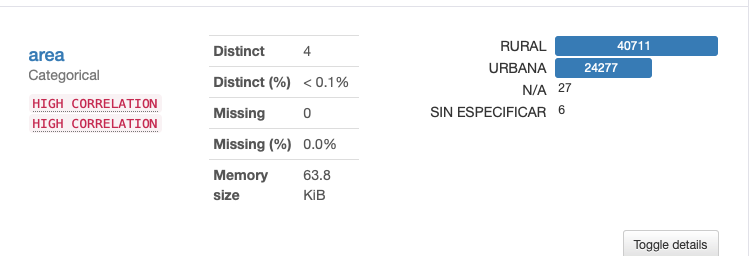
\includegraphics[scale=0.5]{Images/10}
\end{figure}
\end{variable}

%-

\begin{variable}(status) 
Es una variable que representa el status actual del centro educativo, en caso de que se encuentre abierta, cerrado o cualquier otro pormenor.
\bigbreak 
\textbf{Valores posibles.}
\begin{itemize}
	\item 6 variables distintas.
\end{itemize}
\begin{figure}[H]
	\centering
	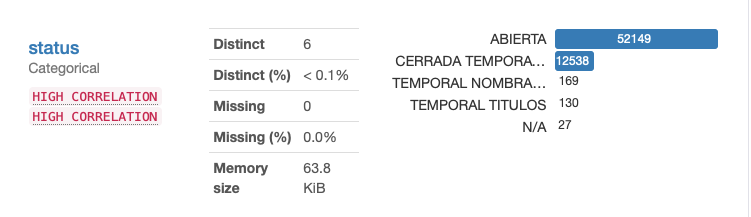
\includegraphics[scale=0.5]{Images/11}
\end{figure}
\end{variable}

%-

\begin{variable}(modalidad) 
Es la modalidad en la que reciben las clases, si se imparten las clases en dos idiomas o solo uno. 
\bigbreak 
\textbf{Valores posibles.}
\begin{itemize}
	\item 3 valores posibles. 
\end{itemize}
\begin{figure}[H]
	\centering
	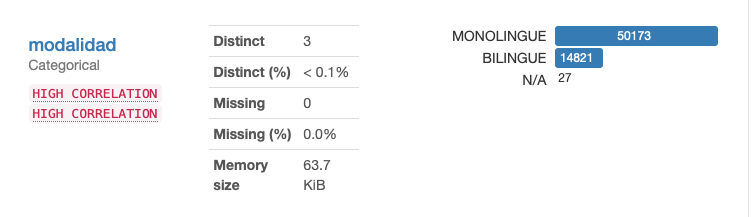
\includegraphics[scale=0.5]{Images/12}
\end{figure}
\end{variable}

%-

\begin{variable}(jornada) 
Es una variable que complementa a la variable de establecimiento ya que separa en una columna específica la jornada del centro educativo.
\bigbreak 
\textbf{Valores posibles.}
\begin{itemize}
	\item 6 datos distintos. 
\end{itemize}
\begin{figure}[H]
	\centering
	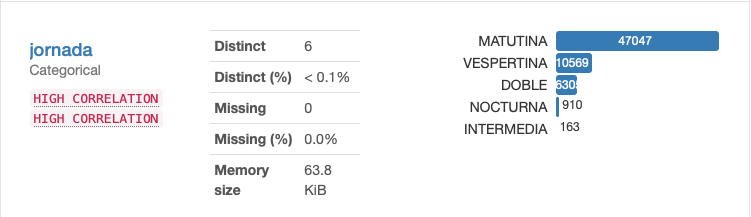
\includegraphics[scale=0.5]{Images/13}
\end{figure}
\end{variable}

%-

\begin{variable}(plan) 
Es una variable que hace referencia al plan en el que se reciben las clases de los centros educativos. 
\bigbreak 
\textbf{Valores posibles.}
\begin{itemize}
	\item 10 datos distintos. 
\end{itemize}
\begin{figure}[H]
	\centering
	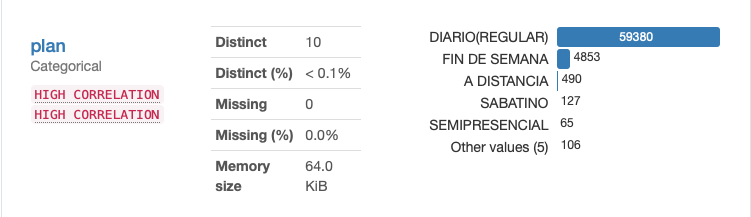
\includegraphics[scale=0.5]{Images/14}
\end{figure}
\end{variable}

%-

\begin{variable}(departamental) 
Es una variable que complementa a los distritos, ya que separa los centros educativos en varias subdivisiones; no necesariamente por departamento geográficos. 
\bigbreak 
\textbf{Valores posibles.}
\begin{itemize}
	\item 27 valores distintos. 
\end{itemize}
\begin{figure}[H]
	\centering
	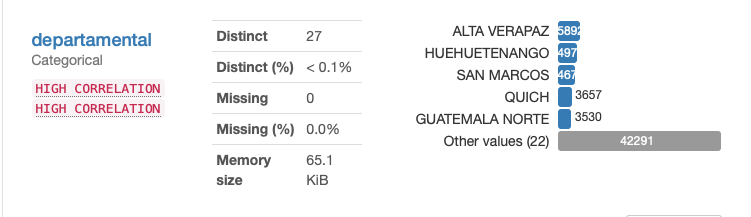
\includegraphics[scale=0.5]{Images/15}
\end{figure}
\end{variable}

%-

\begin{variable}(direccion) 
La dirección es una variable que contiene la dirección exacta de los centros educativos.
\bigbreak 
\textbf{Valores posibles.}
\begin{itemize}
	\item Indeterminado, no parece ser una variable determinando en la base de datos.
\end{itemize}
\begin{figure}[H]
	\centering
	
\includegraphics[scale=0.5]{Images/16}
\end{figure}
\end{variable}

%-

\begin{variable}(telefono) 
El número de teléfono es una variable que representa un medio de comunicación directa al centro educativo. 
\bigbreak 
\textbf{Valores posibles.}
\begin{itemize}
	\item Indeterminado, no parece ser una variable determinante en la base de datos. Esto se produce ya que se intentó tratar como variable categórica. 
\end{itemize}
\begin{figure}[H]
	\centering
	
\includegraphics[scale=0.5]{Images/17}
\end{figure}
\end{variable}













%---------------------------
\bibliographystyle{apa}
\bibliography{referencias.bib}

\end{document}